% ---------------------------------------------------------------------------
% Author guideline and sample document for EG publication using LaTeX2e input
% D.Fellner, v1.13, Jul 31, 2008

\documentclass{egpubl}
\usepackage{pg2014}

% --- for  Annual CONFERENCE
% \ConferenceSubmission % uncomment for Conference submission
% \ConferencePaper      % uncomment for (final) Conference Paper
% \STAR                 % uncomment for STAR contribution
% \Tutorial             % uncomment for Tutorial contribution
% \ShortPresentation    % uncomment for (final) Short Conference Presentation
%
% --- for  CGF Journal
% \JournalSubmission    % uncomment for submission to Computer Graphics Forum
% \JournalPaper         % uncomment for final version of Journal Paper
%
% --- for  CGF Journal: special issue
% \SpecialIssueSubmission    % uncomment for submission to Computer Graphics Forum, special issue
\SpecialIssuePaper         % uncomment for final version of Journal Paper, special issue
%
% --- for  EG Workshop Proceedings
% \WsSubmission    % uncomment for submission to EG Workshop
% \WsPaper         % uncomment for final version of EG Workshop contribution
%
 \electronicVersion % can be used both for the printed and electronic version

% !! *please* don't change anything above
% !! unless you REALLY know what you are doing
% ------------------------------------------------------------------------

% for including postscript figures
% mind: package option 'draft' will replace PS figure by a filename within a frame
\ifpdf \usepackage[pdftex]{graphicx} \pdfcompresslevel=9
\else \usepackage[dvips]{graphicx} \fi

\PrintedOrElectronic

% prepare for electronic version of your document
\usepackage{t1enc,dfadobe}

\usepackage{egweblnk}
\usepackage{cite}

% For backwards compatibility to old LaTeX type font selection.
% Uncomment if your document adheres to LaTeX2e recommendations.
% \let\rm=\rmfamily    \let\sf=\sffamily    \let\tt=\ttfamily
% \let\it=\itshape     \let\sl=\slshape     \l\bfserieset\sc=\scshape
% \let\bf=

% end of prologue

%% ---------------------------------------------------------------------
% EG author guidelines plus sample file for EG publication using LaTeX2e input
% D.Fellner, v1.17, Sep 23, 2010


\title{Minimal Energy Based Hybrid Model For Multi-Agent Simulations}

% for anonymous conference submission please enter your SUBMISSION ID
% instead of the author's name (and leave the affiliation blank) !!
\author{Haiying Liu\thanks{e-mail:lhysunshine@gmail.com}\\Beijing Institute of Technology}


\begin{document}

% \teaser{
%  
\includegraphics[width=\linewidth]{eg_new}
%  \centering
%   \caption{New EG Logo}
% \label{fig:teaser}
% }

\maketitle

\begin{abstract}
   The behavior of large human crowd is very complicated and subtle due to complex local collision strategies for dynamic crowd density distribution in the scene. We present a hybrid approach to simulate complex crowd behavior by combining continuous crowd algorithm and agent-based algorithm. For dense groups, we introduce a minimal-energy method to minimize conflict between dense groups and constrain the maximum density of each grid; For sparse groups, we adapt RVO algorithm to simulate agent-agent and agent-group interactions.

\begin{classification} % according to http://www.acm.org/class/1998/
\CCScat{Computer Graphics}{I.3.7}{Three-Dimensional Graphics and Realism}{Animation}
\end{classification}

\end{abstract}





%-------------------------------------------------------------------------
\section{Introduction}

Please follow the steps outlined in this document very carefully when
submitting your manuscript to Eurographics.

You may as well use the \LaTeX\ source as a template to typeset your own
paper. In this case we encourage you to also read the \LaTeX\ comments
embedded in the document.

%-------------------------------------------------------------------------
\section{Related Work}

\section{Dense Crowd Flow Energy Minimization}

In this section, we introduce our approach of minimizing collision energy of dense crowds. In the observation of dense crowds behavior, groups of agents have inter-group collision, merging and negotiation while the freedom of movement of individual agents are reduced\cite{Treuille:2006,Narain:2009,Golas:2013}. Based on the observation, we define two types of collision energy, inter-group and inter-agent collision energy. We use the continuous dense crowd model from \cite{Narain:2009} to represent and minimize inter-agent collision behavior(\S\ref{section:3.1}). We develop our inter-group energy model and employ Graph Cut to minimize inter-group collision energy(\S\ref{section:3.2}). Besides, we introduce a series of constraints to limit maximum density of each group(\S\ref{section:3.3}). 

\subsection{Dense Crowd Representation}
\label{section:3.1}
Like \cite{Narain:2009}, we first use Navigation Mesh as global planning algorithm for each agent(see for details). Then, the information of discrete agents is transfered to grids by the particle-in-cell method of fluid simulation \cite{Narain:2009}. The density $\rho$ and velocity $\bar{\textbf{v}}$ can be computed as,
\begin{equation}
\label{eq:1}
 \rho(\textbf{x}) = \sum_{i} \omega_\textbf{x}(\textbf{x}_i)m_i
\end{equation}
\begin{equation}
\label{eq:2}
 \bar{\textbf{v}}(\textbf{x}) = \frac{\sum_{i} \omega_\textbf{x}(\textbf{x}_i)\tilde{\textbf{v}}_i}{\sum_{i} \omega_\textbf{x}(\textbf{x}_i)}
\end{equation} 
where $\textbf{x}_i$ is the position of the agent, $\tilde{\textbf{v}}_i$ is the prefered velocity of the agent, $m_i$ is the mass of each agent which are unity. $\omega_\textbf{x}(\textbf{x}_i)$ is the bilinear interpolation weight associated with the agent position.

After the crowd is converted to continuous representation, we can refine the crowd information by minimizing the inter-group collision energy descripted in (\S\ref{section:3.2} and \S\ref{section:3.3}).

Then, the density $\rho(\textbf{x}_i)$ and velocity $\textbf{v}(\textbf{x}_i)$ at agent position can be interpolated from grid density and grid velocity with the same method mentioned in \cite{Treuille:2006}. We can get the final velocity of each agent by interpolation between the continuum velocity $\textbf{v}(\textbf{x}_i)$ and the agent's prefered velocity $\tilde{\textbf{v}}_i$, depending on the crowd density $\rho(\textbf{x}_i)$ at its location:
\begin{equation}
\label{eq:3}
\textbf{v}_i = \tilde{\textbf{v}}_i + \frac{\rho(\textbf{x}_i)}{\rho_{max}}(\textbf{v}(\textbf{x}_i) - \tilde{\textbf{v}}_i)
\end{equation}

\subsection{Energy Minimization Model}
\label{section:3.2}
According to our observation of dense crowd behavior, collisions, merging and negotiations happen between agent groups in dense crowds. However, not like local collision avoidance strategies for agents which can be considered as rigid-body, groups are highly influenced by neighbor groups and have the trend of sharing the same movement. Inspired by the observation, we develop a minimal energy model to describe and solve inter-group collision problem.

\begin{figure}
\centering
  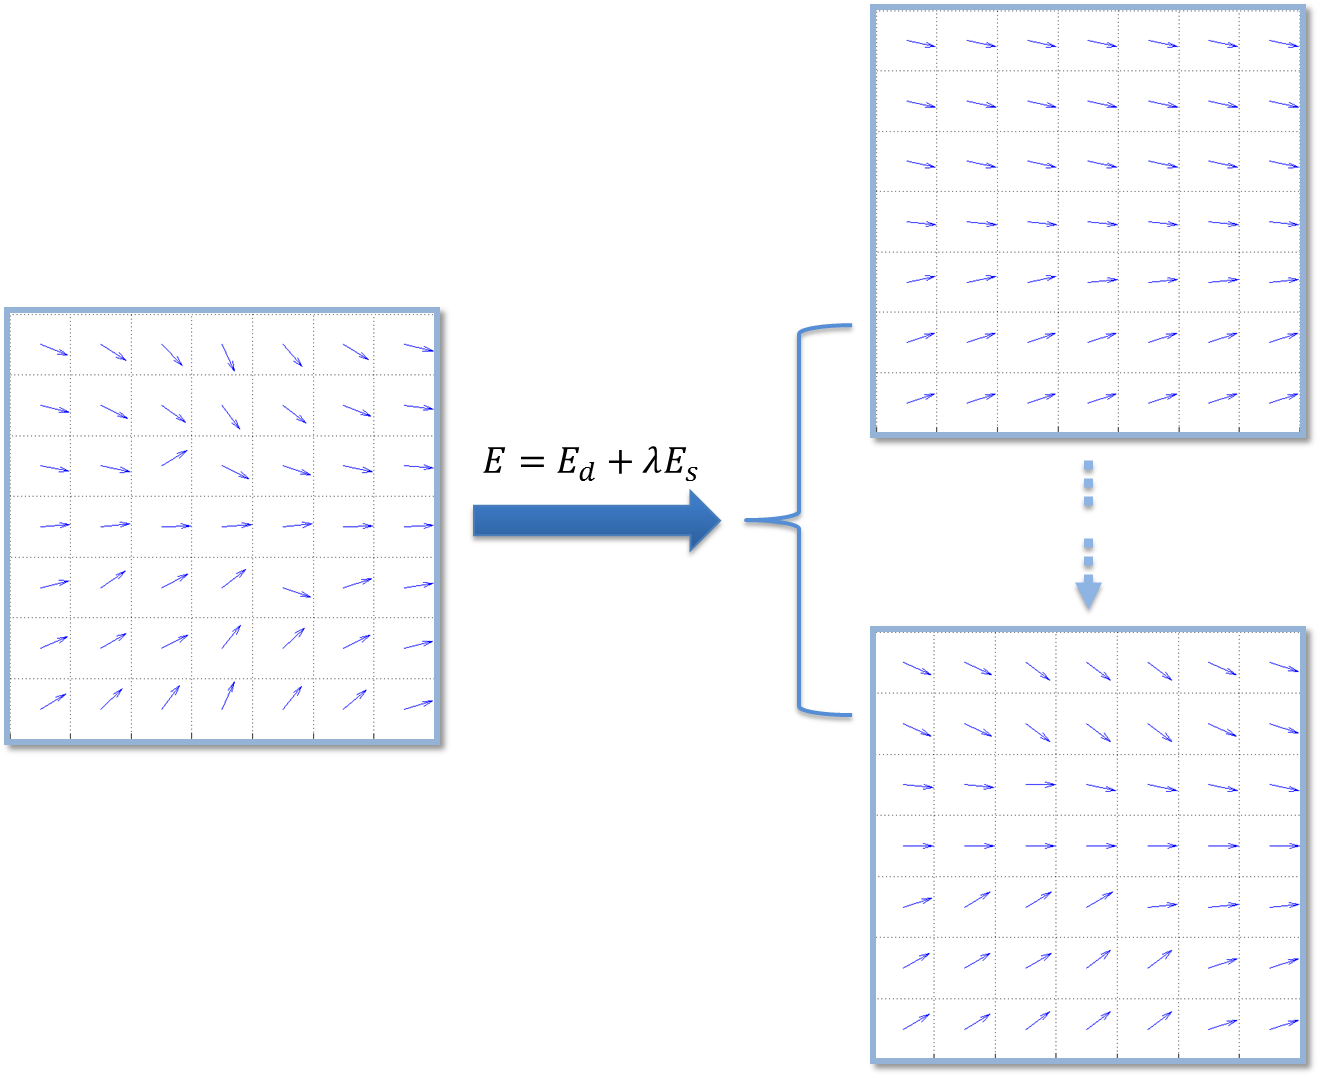
\includegraphics[width=3in]{images/energy}
  \caption{Minimal-Engergy Process Illustration. The left image is group of dense grids with grid velocities. Images on the right side are grids with refined velocities. From right-top to right-bottom, the $\lambda$ of smooth term decreased which means each grid is less influenced by neighbor grids.}
\end{figure}
We define the inter-group collision problem as a labelling problem by assigning to each grid $i$ a label $l_i$. Each grid maps to a group of agent and the number of grids are $n$. By dividing space into $m$ pieces, we can have $m$ labels, each of them represent a range of angle in the space. The energy function $E$, composed of a data energy $E_d$ and a smoothness energy $E_s$, is defined as:
\begin{equation}
\label{eq:4}
E = E_d + \lambda E_s
\end{equation}

The data energy $E_d$ is the sum of data cost of each grid with a label $d_i(l_i)$. In our energy model, the data cost $d_i(l_i)$ is defined as the angular distance from the average grid velocity $\bar{\textbf{v}}(\textbf{x})$ to the velocity of selected label $\hat{\textbf{v}}(l_i)$, which means the effort of the group to change it's velocity to negotiate with neighbor groups. We first normalize the two velocities and use the dot value of them in our implementation instead of computing angular difference as equation \ref{eq:6}.
\begin{equation}
\label{eq:5}
E_d = \sum_{i}d_i(l_i)
\end{equation}

\begin{equation}
\label{eq:6}
d_i(l_i) = 1 - \bar{\textbf{v}}(\textbf{x}) \cdot \hat{\textbf{v}}(l_i)
\end{equation}

The smoothness energy $E_s$ represent the velocity difference between neighbor grids. We use standard 4 neighbor system for dense grids, so that the smoothness energy is the sum of spacially varying horizontal and vertical neighbor smoothness costs $V_{ij}(l_i,l_j)$, where if $i=(p,q)$ and $j=(s,t)$ then $\left|p-s\right| + \left|q-t\right| = 1$. Let $\mathcal{N}$ denotes the set of all such neighboring grid pairs, the smoothness energy is
\begin{equation}
\label{eq:7}
E_s = \sum\limits_{\left\{ {i,j} \right\} \in \mathcal{N}} \omega_{ij} \cdot V(\left|l_i,l_j\right|)
\end{equation}

In equation \ref{eq:7}, $V(\left|l_i,l_j\right|)$, also can be written as $V(\Delta l)$, is a non-decreasing fundtion of the label difference, and can be directly computed as absolute differenct between two labels. $\omega_{ij}$ is a per-pair weight for $i$th and $j$th grid, which is normalized by the minimum density of a dense grid $\rho_{min}$ and the maximum density $\rho_{max}$ (see equation \ref{eq:8}). In our model, $V(\left|l_i,l_j\right|)$ is adapted to restrict the maximum density of each group(\S\ref{section:3.3}).
\begin{equation}
\label{eq:8}
\omega_{ij} = \frac{(\rho_i - \rho_{min})(\rho_j - \rho_{min})}{(\rho_{max} - \rho_{min})^2}
\end{equation}

With the definition of energy function $E$, we can use Graph Cut or Belief Propagation algorithms to compute labels for each grid to achieve the minimal energy cost. In our implementation, we use the Graph Cut implementation from \cite{Boykov:2001,Boykov:2004,Kolmogorov:2004}.

\subsection{Constraints}
\label{section:3.3}
While trying to reach the minimal energy cost of inter-group collision, we should also keep the density of each group below the maximum density $\rho_{max}$ because of the incompressibility of human body. If the density of the grid $i$ is below $\rho_{max}$, agents can be pushed into the grid from neighbor grids. When the density of the grid $i$ is greater than $\rho_{max}$, the the grid is incompressible. The smooth term should be,
\begin{equation}
\label{eq:9}
V(\left|l_i,l_j\right|) = \left\{ 
{\begin{array}
{*{20}{c}}
{\alpha \left| {{l_i} - {l_j}} \right|,  {\rho _i} \le {\rho _{max}}}\\
{\Delta _{max},  {\rho _i} > {\rho _{max}}}
\end{array}} 
\right.
\end{equation}
where $\Delta_{max}$ is a constant value as a penalty of labels which could lead to potential overcrowded (see in Figure \ref{figure:grid_constraints}).

\begin{figure}
\label{figure:grid_constraints}
  \centering
  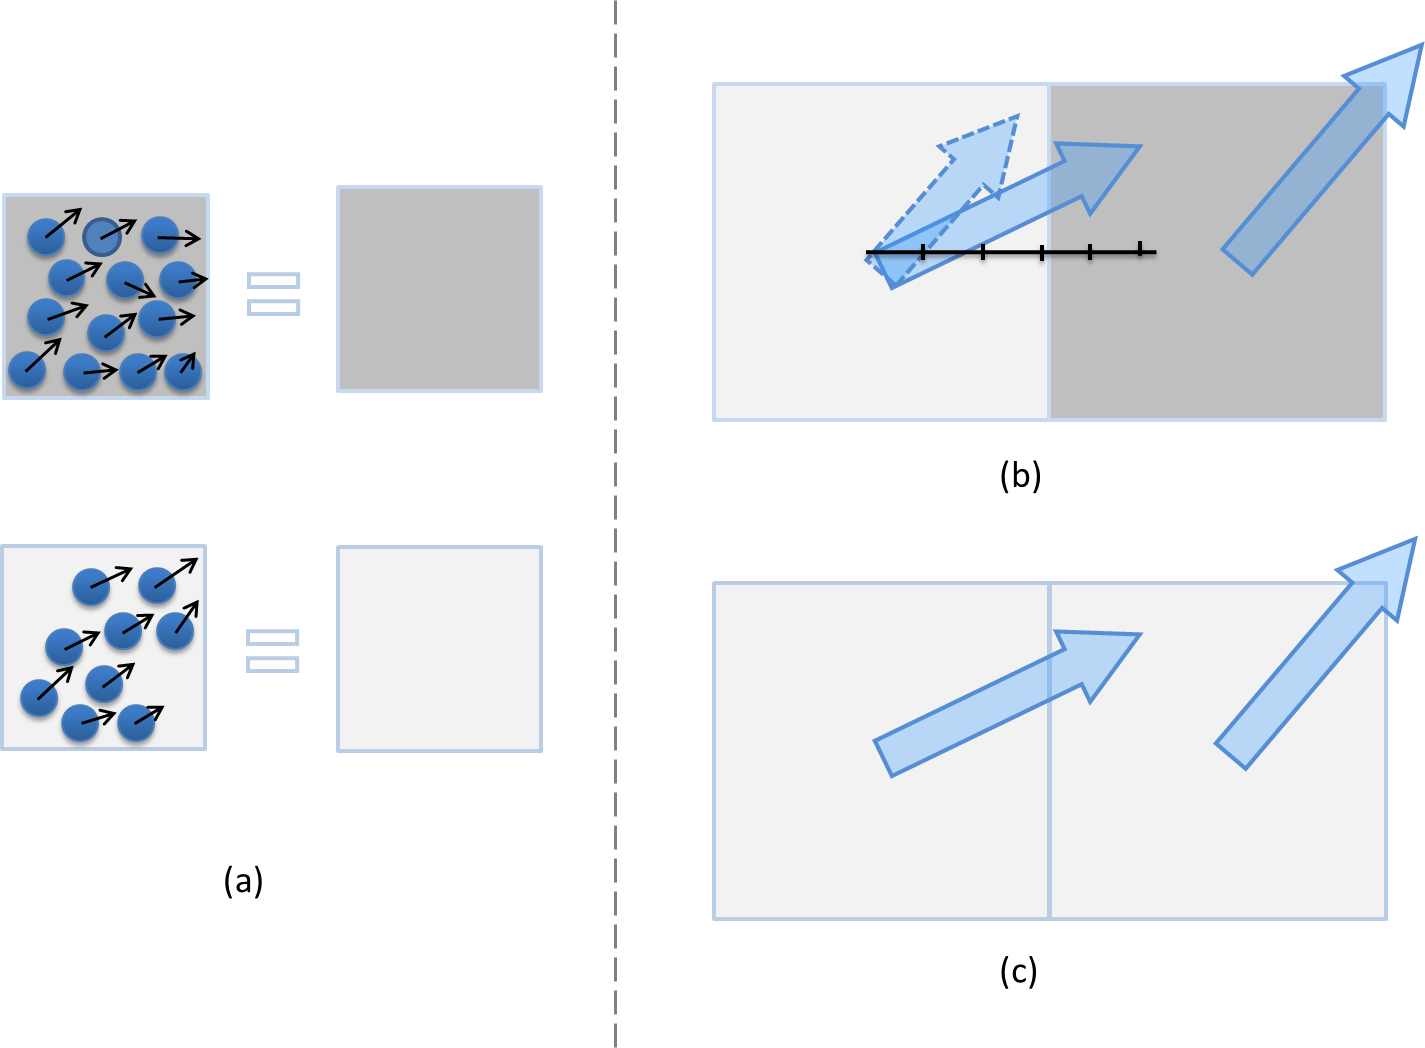
\includegraphics[width=3in]{images/fig_inter_grid_constraints}
  \caption{Sample illustration.}
\end{figure}

\section{Hybrid Crowd Simulation}
Continuous crowd methods and agent-based methods are both based on assumptions of agent number and crowd density(see \ref{Golas:2013}).
\begin{figure*}
  \centering
  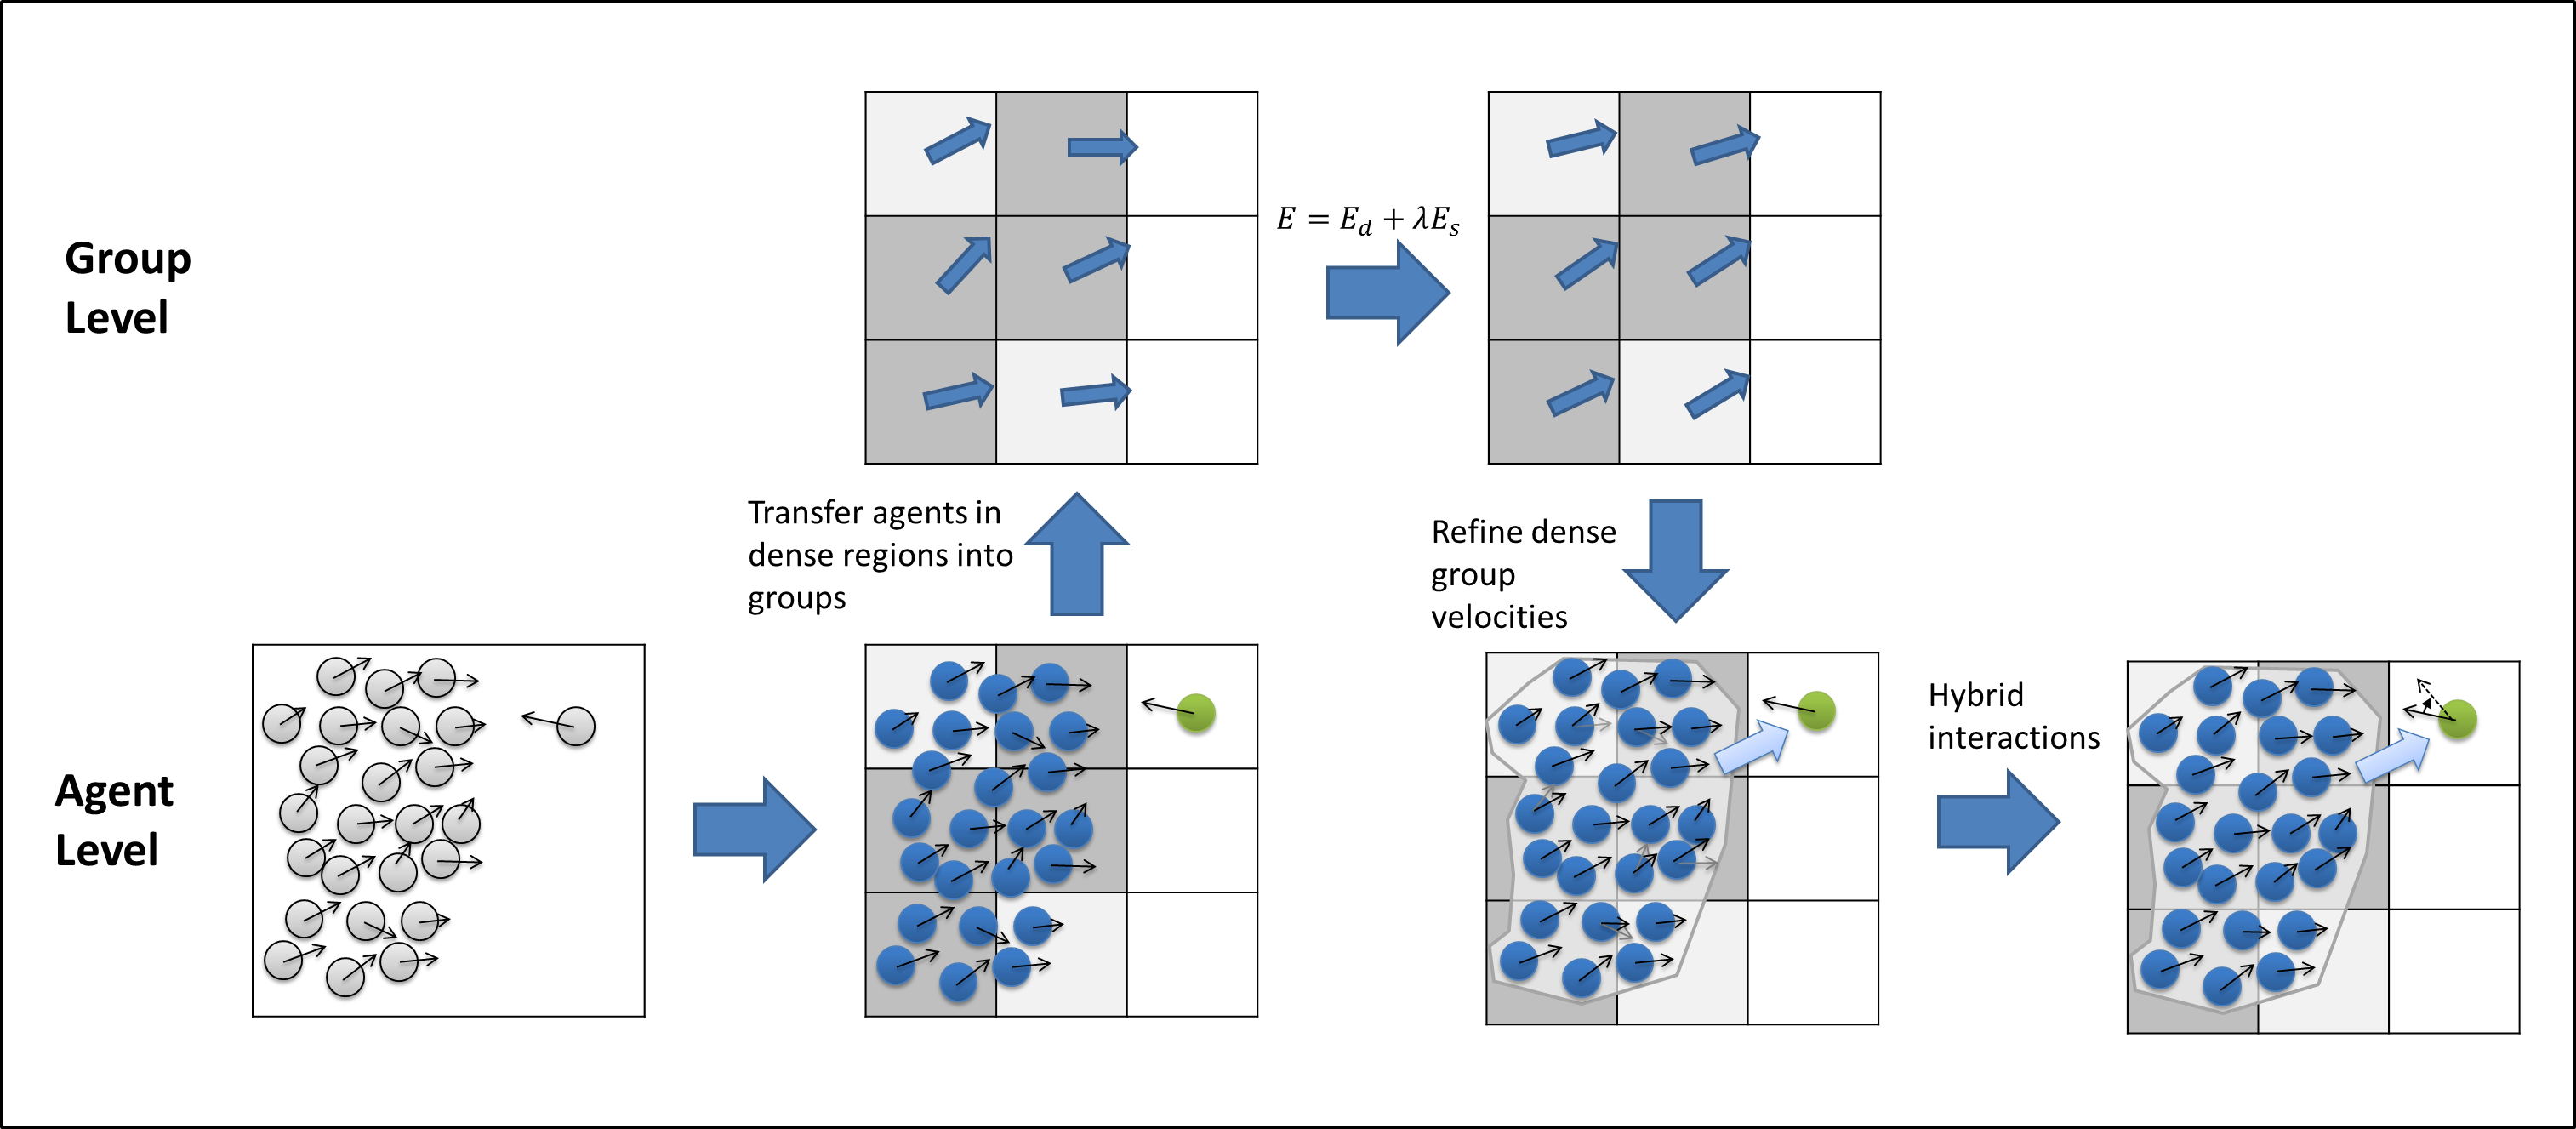
\includegraphics[width=6.4in]{images/pipeline}
  \caption{Sample illustration.}
\end{figure*}

\subsection{Dense Crowd Silhouette}

\subsection{Agent-based}
\begin{figure}
\centering
  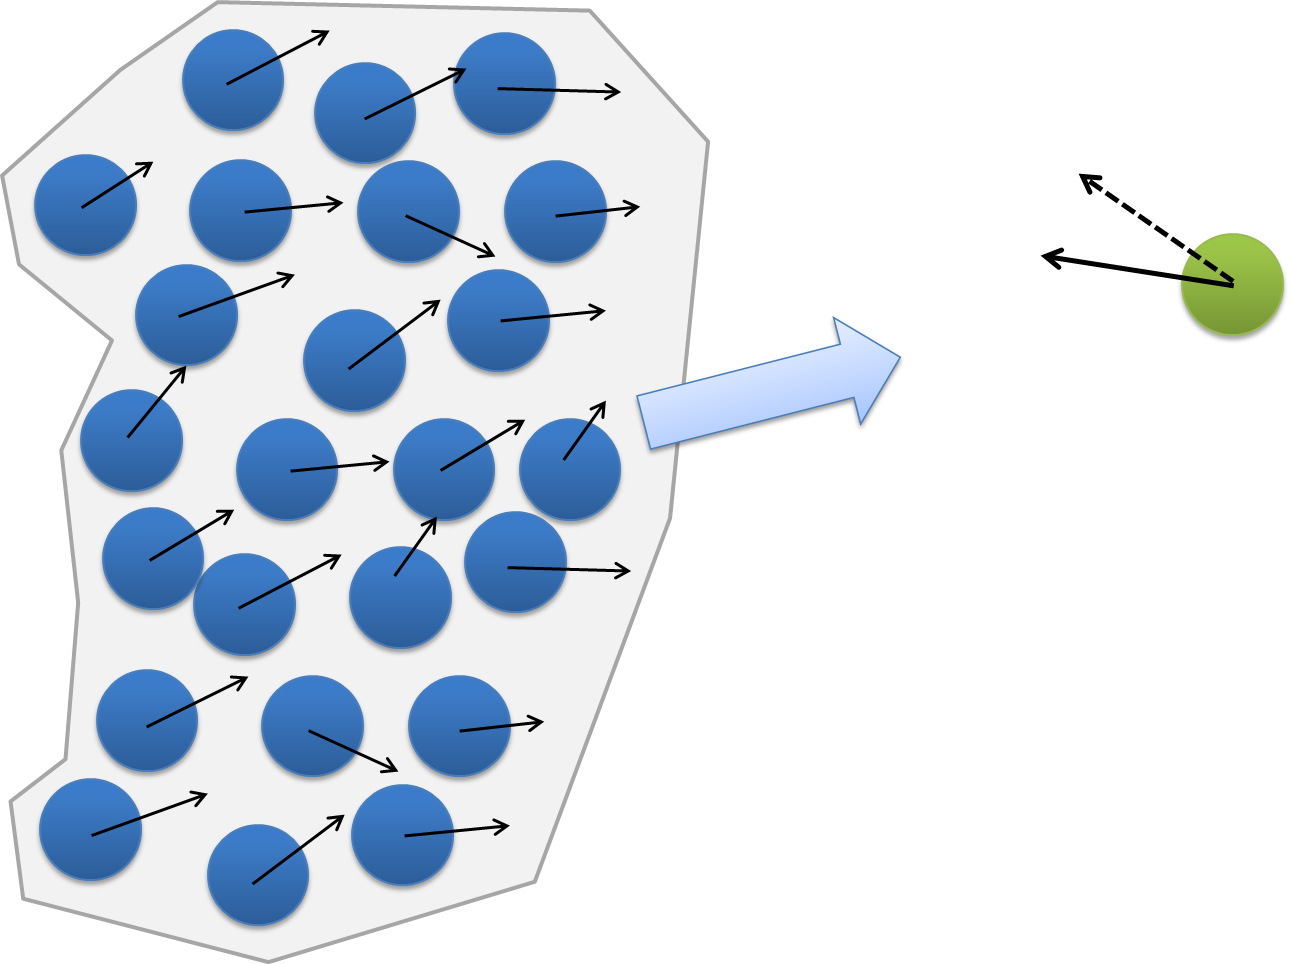
\includegraphics[width=1.6in]{images/agent_group_collision}
  \caption{Sample illustration.}
\end{figure}

%\bibliographystyle{eg-alpha}
\bibliographystyle{eg-alpha-doi}

\bibliography{reference}
\end{document}

% ---------------------------------------------------------------------
% EG author guidelines plus sample file for EG publication using LaTeX2e input
% D.Fellner, v1.17, Sep 23, 2010


\title{Minimal Energy Based Hybrid Model For Multi-Agent Simulations}

% for anonymous conference submission please enter your SUBMISSION ID
% instead of the author's name (and leave the affiliation blank) !!
\author{PaperID-1122}


\begin{document}

% \teaser{
%  
\includegraphics[width=\linewidth]{eg_new}
%  \centering
%   \caption{New EG Logo}
% \label{fig:teaser}
% }

\maketitle

\begin{abstract}

The behavior of large human crowd is very complicated and subtle due to complex local collision strategies for varying crowd density distribution in the scene. We present a hybrid approach to simulate complex crowd behavior by combining continuous crowd algorithm and agent-based algorithm. For dense groups, we introduce a minimal-energy method to minimize conflict between dense groups and constrain the maximum density of each grid; For sparse groups, we adapt RVO algorithm to simulate agent-agent and agent-group interactions.

\begin{classification} % according to http://www.acm.org/class/1998/
\CCScat{Computer Graphics}{I.3.7}{Three-Dimensional Graphics and Realism}{Animation}
\end{classification}

\end{abstract}

%-------------------------------------------------------------------------
\section{Introduction}

The simulation of human crowds in realistic interactive scenes is a necessary and challenging task. Crowd simulation technologies have been widely applied in social psychology, transportation research and architecture. There are two major branches in crowd simulation research field, agent-based methods and continuous crowd methods. For agent-based methods, the total number of agents and density of the crowd are restrict due to the computational bottleneck. Continuous crowd methods which based on assumptions of medium to large crowd, suffer from poorer performance in low density regions.

In this paper, we focus on the problem of simulating crowds under varying densities. In high density regions, the movement of each agent are highly restricted and influenced by neighbour agents. From the macroscopic view, the movement of the crowd is driven by collision and cooperation between groups instead of individual will of each agent \cite{Narain:2009}. We define this kind of behaviour as group-group interaction. In low density regions, agents have higher freedom of movement. The collision avoidance decision of each agent is based on its neighbor agents and goal. We define behaviors like this as agent-agent interaction, which is a very common assumption in agent-based methods \cite{Guy:2009,VDBerg:2011,Ondrej:2010}. Besides, there's a third type of behavior which we defined as agent-group interaction. We can see agent-group interactions happen in the boundary of dense crowds where individual agents outside the crowd may choose to join or avoid the crowd. Based on such observation, we develop a hybrid model to choose proper algorithm for each agent and integrate continuous crowd simulation result with agent-based simulation process to support all the agent-agent, agent-group and group-group interactions. 

We proposed a novel minimal-energy based method to simulate interactions between dense groups. A dense group is a small set of agents sharing a common neighbourhood. As for each group, the influence from neighbour groups is similar to label yielding process, we consider the collision and cooperation between groups as a labelling problem. With the formulation we proposed to adapt group-group interaction into labelling problem, Graph-Cut or Belief Propagation which has been successfully used in stereo matching, image restoration and optical flow \cite{Pedro:2004,Marshall:2003,Qingxiong:2009}, can be applied to solve the problem of dense crowd simulation. 

The key contribution of this work can be summarized as follows:
\begin{itemize}
\item a hybrid model combining continuous crowd algorithm and agent-based algorithm for varying densities crowd to simulate interactions between agents and groups. \S\ref{section:4}
\item a minimal-energy model which reduces the dense group collision energy to model interactions between groups. \S\ref{section:3}
\end{itemize}

We demonstrate the quality and performance of agent-group and group-group interactions simulated by our approach on two senarios. Our approach has a small computational cost and can simulate thousands of agents interactively on a single-core CPU. More analysis of our approach can be found in \S\ref{section:5}. 

\begin{figure*}
  \centering
  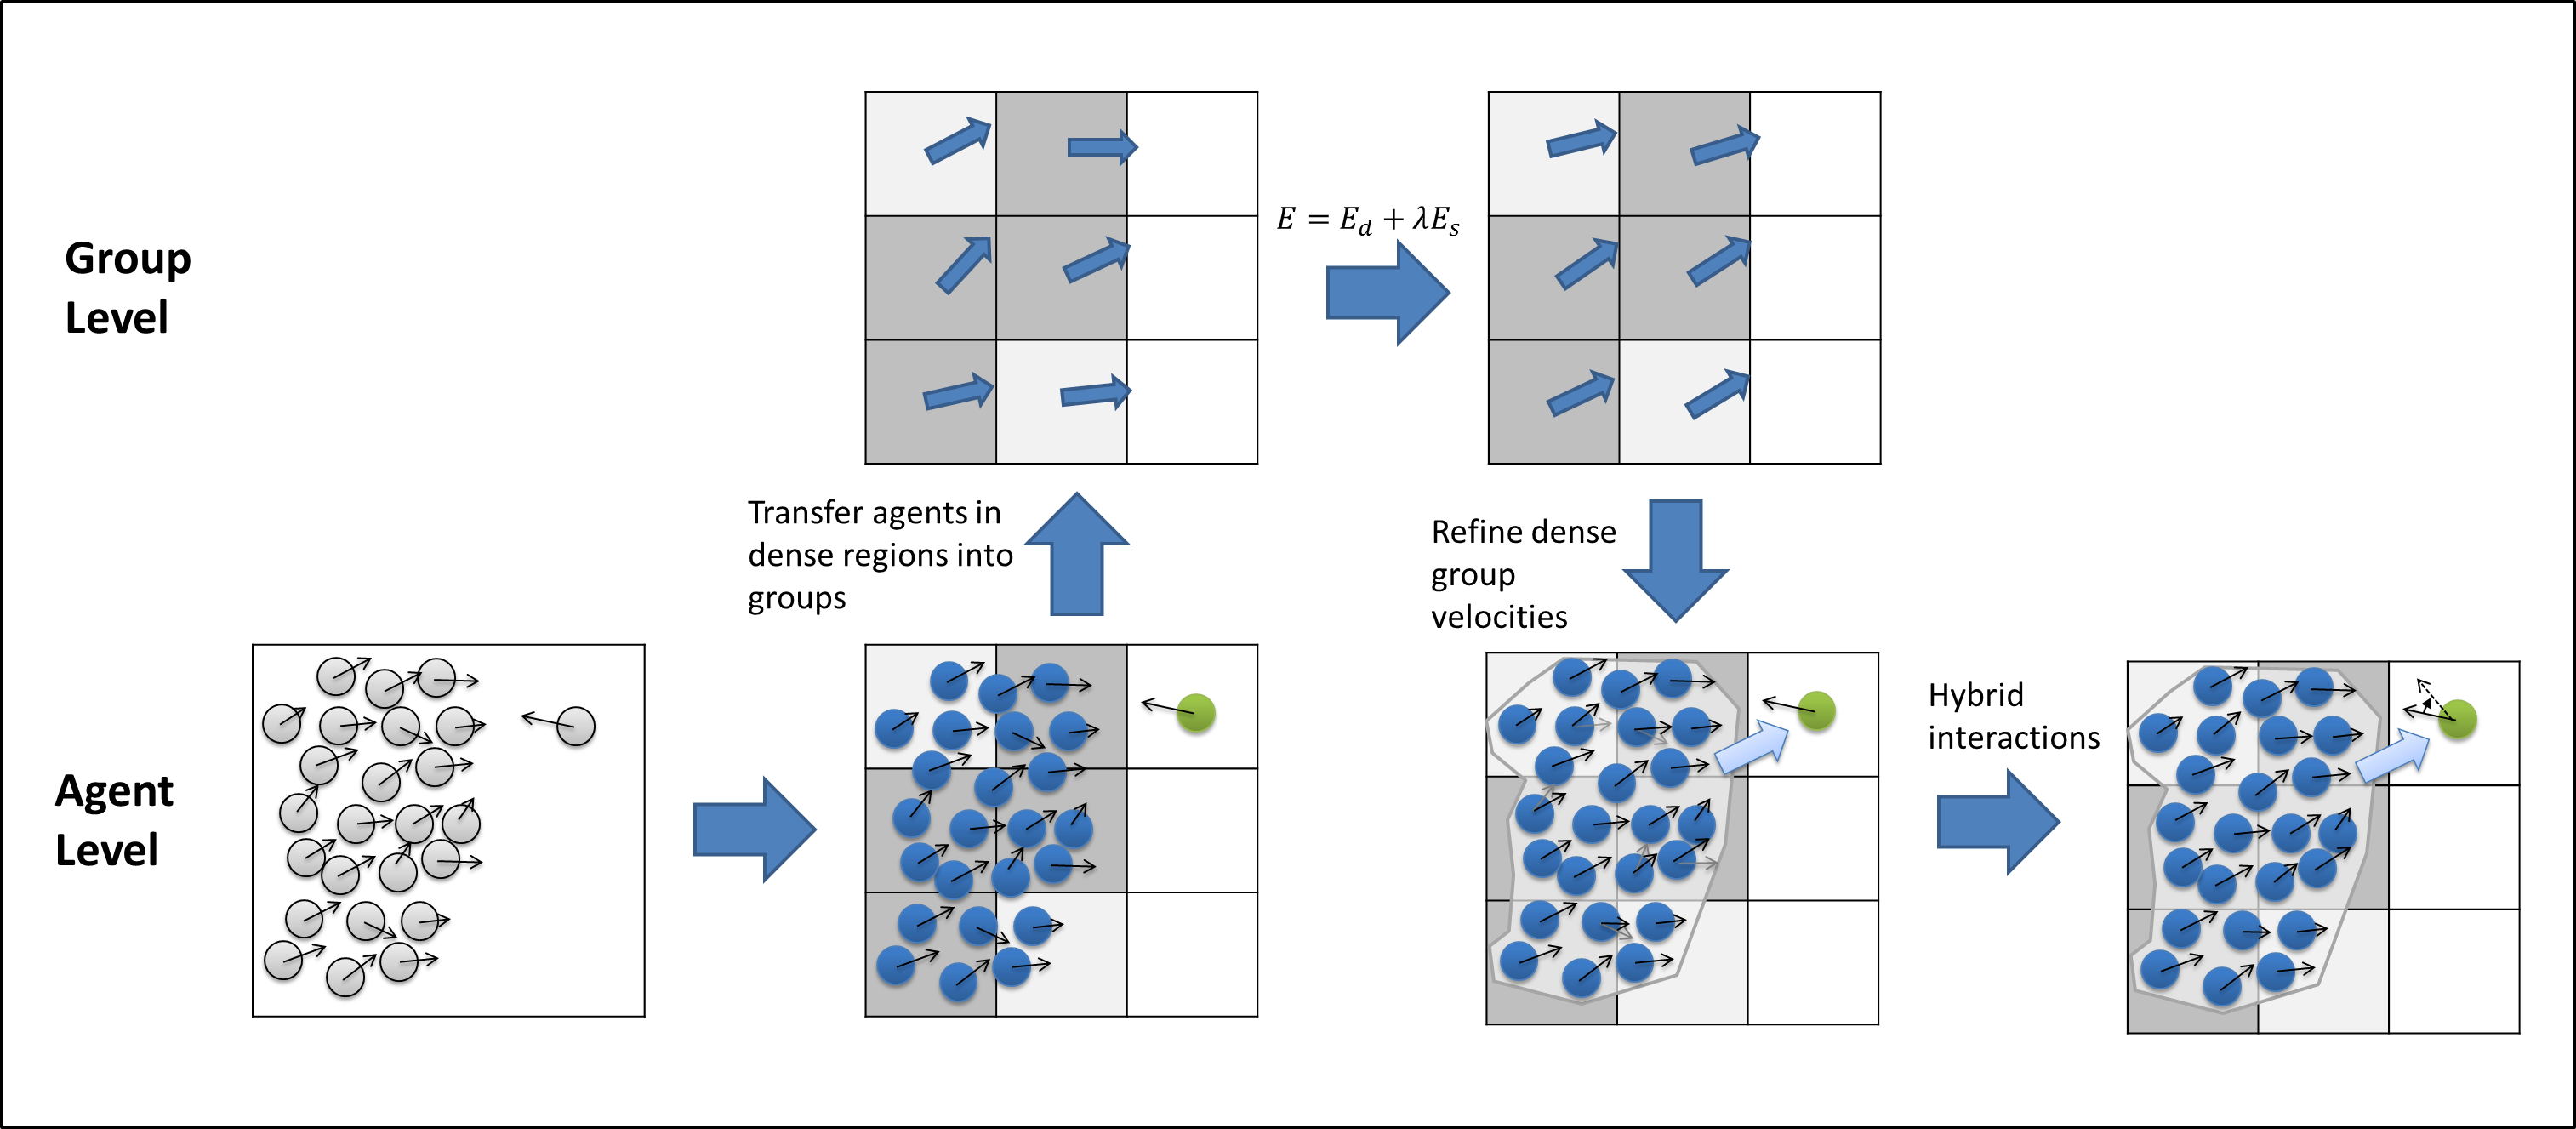
\includegraphics[width=6.4in]{images/pipeline}
  \caption{Hybrid Model Pipeline.}
  \label{fig:pipeline}
\end{figure*}

%-------------------------------------------------------------------------
\section{Related Work}
In this section, we give a brief overview of prior work of crowd simulation and multi-agent system. There are two steps, navigation and collision avoidance in most crowd simulation systems. Navigation, also been called as global-planning, is the process to find a path from the current agent position to the goal that avoid collision with static obstacles in the scene. There're lots of work on this topic \cite{Funge:1999,Bayanzit:2002,Lamarche:2004,Sud:2007,Sud:2008}. We don't go for details of previous work in this aspect.

Collision avoidance is another hot topic with a large amount of works been proposed. One of the traditional ways to classify collision avoidance methods is based on the representation of crowds, either discrete or continuous. In discrete representation, also called as agent-based representation, the collision avoidance decision is made by each individual agent respect to the other agents and obstacles. A number of different models like social forces \cite{Helbing:1995,Helbing:2005,Gayle:2009,Sud:2007}, socialogical factors \cite{Musse:1997}, psychological factors \cite{Pelechano:2008} and synthetic-vision based steering \cite{Ondrej:2010} were used to formulate the collision avoidance behavior of agents. There're also a lot number of methods based on spatial and geometric relationships between agents \cite{VDBerg:2008,VDBerg:2009,Guy:2009,VDBerg:2011}. As geometrically-based methods showed very good quality and became very popular these years, many other models were adapted into these methods for further quality improvement and more complicated agent behavior simulation, like least effort energy model \cite{Guy:2010}, personality traits model \cite{Guy:2011} and stress model \cite{Kim:2012}. Although agent-based methods works quite good in many situations, they suffer from the poor performance with dense crowds.

In continuous representation, agents are influenced by their dense neighbourhood and have less freedom to make independent collision avoidance decisions. Continuum theory for pedestrians flow was first proposed by \cite{Hughes:2003} and extended by \cite{Treuille:2006}. The approach of \cite{Treuille:2006} combined global planning and local collision avoidance into a single pipeline and provided good performance for medium size crowd with a common goal. However, this approach is not suitable for tightly packed crowds and varying goals. The state-of-art work of continuous methods is \cite{Narain:2009}, which combined a Lagrangian representation of individuals with a coarser Eulerian crowd model to capture discrete motion of individual agents and macroscopic flow of crowds. The work of \cite{Narain:2009} can simulate great number of agents at interactive rates and have good performance on dense crowds. However, continuous methods fail to provide accurate results in low density regions as the assumptions of density are no longer hold. 

To make good use of advantages of both methods and avoid the drawbacks, a hybridization of those two methods could be a good solution. \cite{Golas:2013} presented a long range collision avoidance model which can work with both agent-based and continuous representations. Unlike their work, our approach focus on more complicated crowd behavior including agent-agent, agent-group and group-group interactions. We can simulate different crowd behaviors, e.g. whether a agent join or avoid a crowd in front, by simply changing parameters in our hybrid model system. 


%-------------------------------------------------------------------------
\section{Dense Crowd Flow Energy Minimization}
\label{section:3}

In this section, we introduce our approach of minimizing collision energy of dense crowds. In the observation of dense crowds behavior, groups of agents have inter-group collision, merging and negotiation while the freedom of movement of individual agents are reduced\cite{Treuille:2006,Narain:2009,Golas:2013}. Based on the observation, we define two types of collision energy, inter-group and inter-agent collision energy. We use the continuous dense crowd model from \cite{Narain:2009} to represent and minimize inter-agent collision behavior(\S\ref{section:3.1}). We develop our inter-group energy model and employ Graph Cut to minimize inter-group collision energy(\S\ref{section:3.2}). Besides, we introduce a series of constraints to limit maximum density of each group(\S\ref{section:3.3}). 

\subsection{Dense Crowd Representation}
\label{section:3.1}

Like \cite{Narain:2009}, we first use Navigation Mesh as global planning algorithm for each agent(see for details). Then, the information of discrete agents is transfered to grids by the particle-in-cell method of fluid simulation \cite{Narain:2009}. The density $\rho$ and velocity $\bar{\textbf{v}}$ can be computed as,
\begin{equation}
\label{eq:1}
 \rho(\textbf{p}) = \sum_{i} \omega_\textbf{p}(\textbf{p}_i)m_i
\end{equation}
\begin{equation}
\label{eq:2}
 \bar{\textbf{v}}(\textbf{p}) = \frac{\sum_{i} \omega_\textbf{p}(\textbf{p}_i)\tilde{\textbf{v}}_i}{\sum_{i} \omega_\textbf{p}(\textbf{p}_i)}
\end{equation} 
where $\textbf{x}_i$ is the position of the agent, $\tilde{\textbf{v}}_i$ is the prefered velocity of the agent, $m_i$ is the mass of each agent which are unity. $\omega_\textbf{p}(\textbf{p}_i)$ is the bilinear interpolation weight associated with the agent position.

After the crowd is converted to continuous representation, we can refine the crowd information by minimizing the inter-group collision energy descripted in (\S\ref{section:3.2} and \S\ref{section:3.3}).

Then, the density $\rho(\textbf{p}_i)$ and velocity $\textbf{v}(\textbf{p}_i)$ at agent position can be interpolated from grid density and grid velocity with the same method mentioned in \cite{Treuille:2006}. We can get the final velocity of each agent by interpolation between the continuum velocity $\textbf{v}(\textbf{p}_i)$ and the agent's prefered velocity $\tilde{\textbf{v}}_i$, depending on the crowd density $\rho(\textbf{p}_i)$ at its location:
\begin{equation}
\label{eq:3}
\textbf{v}_i = \tilde{\textbf{v}}_i + \frac{\rho(\textbf{p}_i)}{\rho_{max}}(\textbf{v}(\textbf{p}_i) - \tilde{\textbf{v}}_i)
\end{equation}

\subsection{Energy Minimization Model}
\label{section:3.2}

According to our observation of dense crowd behavior, collisions, merging and negotiations happen between agent groups in dense crowds. However, not like local collision avoidance strategies for agents which can be considered as rigid-body, groups are highly influenced by neighbor groups and have the trend of sharing the same movement. Inspired by the observation, we develop a minimal energy model to describe and solve inter-group collision problem.

\begin{figure}
\centering
  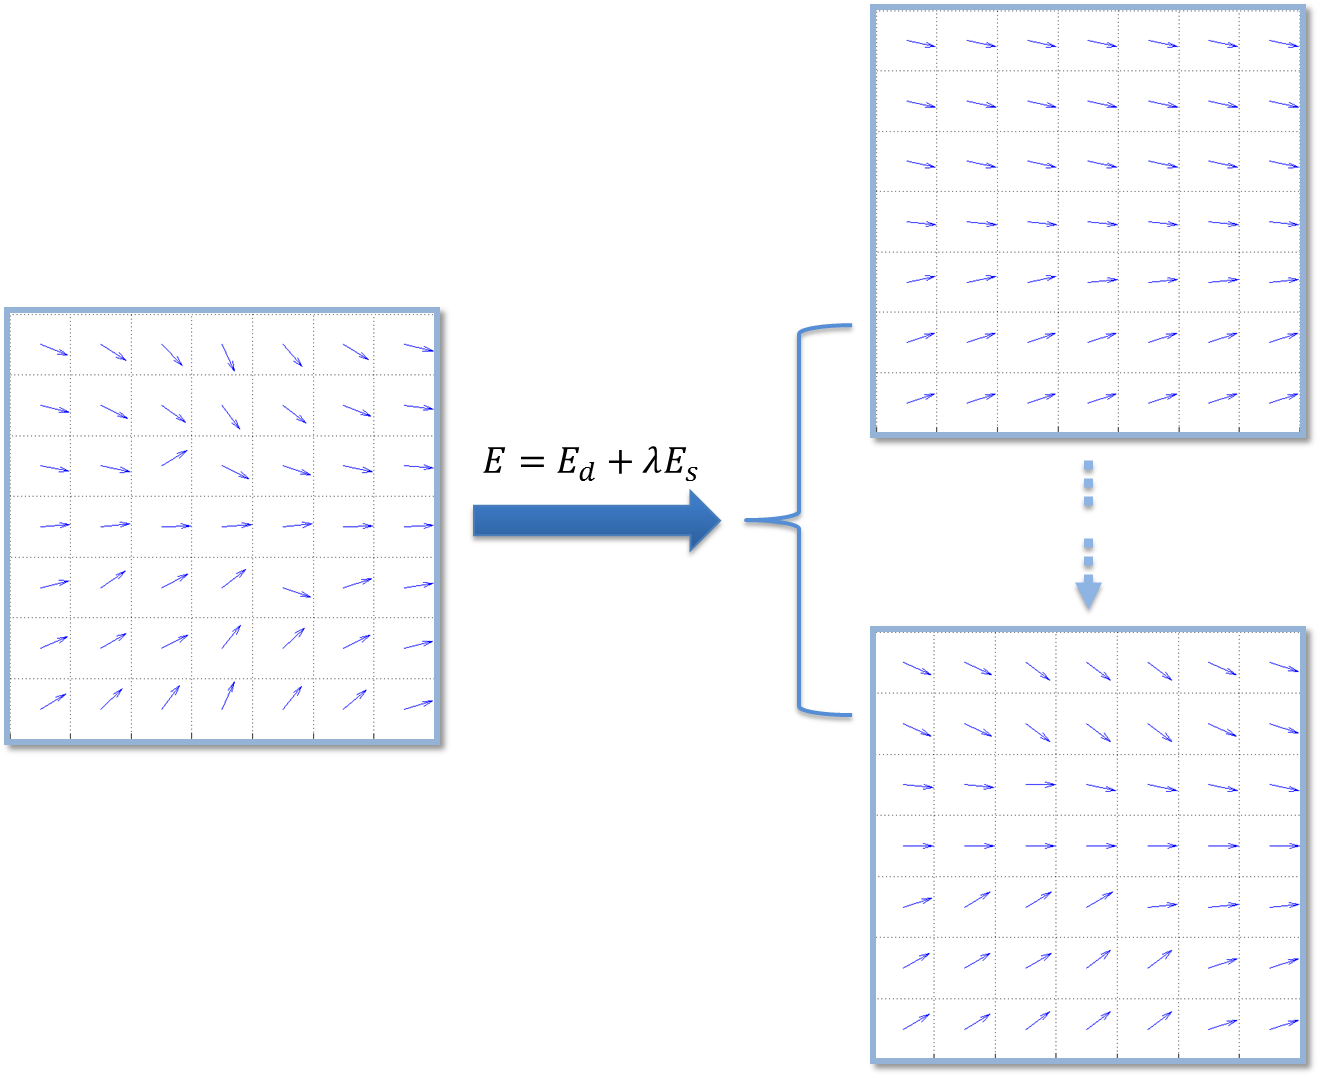
\includegraphics[width=3in]{images/energy}
  \caption{Minimal-Engergy Process Illustration. The left image is group of dense grids with grid velocities. Images on the right side are grids with refined velocities. From right-top to right-bottom, the $\lambda$ of smooth term decreased which means each grid is less influenced by neighbor grids.}
  \label{fig:energy_model}
\end{figure}

We define the inter-group collision problem as a labelling problem by assigning to each grid $i$ a label $l_i$. Each grid maps to a group of agent and the number of grids are $n$. We call the energy minimization process twice to mininize collision energy of horizontal and vertical direction seperately. For each optimization pass, we can have $m$ labels by dividing horizontal or vertical space into $m$ pieces, each of them represent a segment x or y axis. The energy function $E$, composed of a data energy $E_d$ and a smoothness energy $E_s$, is defined as:
\begin{equation}
\label{eq:4}
E = E_d + \lambda E_s
\end{equation}

The data energy $E_d$ is the sum of data cost of each grid with a label $d_i(l_i)$. In our energy model, the data cost $d_i(l_i)$ is defined as the absolute distance between projection on x or y axis of the average grid velocity $\bar{\textbf{v}}(\textbf{p})$ , and the value of selected label which means the effort of the group to change it's velocity on x or y axis to certain label.
\begin{equation}
\label{eq:5}
E_d = \sum_{i}d_i(l_i)
\end{equation}


The smoothness energy $E_s$ represents the velocity difference between neighbor grids. We use standard 4 neighbor system for dense grids, so that the smoothness energy is the sum of spacially varying horizontal and vertical neighbor smoothness costs $V_{ij}(l_i,l_j)$, where if $i=(p,q)$ and $j=(s,t)$ then $\left|p-s\right| + \left|q-t\right| = 1$. Let $\mathcal{N}$ denotes the set of all such neighboring grid pairs, the smoothness energy is
\begin{equation}
\label{eq:6}
E_s = \sum\limits_{\left\{ {i,j} \right\} \in \mathcal{N}} V(\left|l_i,l_j\right|)
\end{equation}

In equation \ref{eq:6}, $V(\left|l_i,l_j\right|)$, also can be written as $V(\Delta l)$, is a non-decreasing function of the label difference, and can be directly computed as absolute differenct between two labels. The scale value $\lambda$ in Equation \ref{eq:4} can be used to control the influence by neighbors. We can see the different optimization result by changing $\lambda$ in Figure \ref{fig:energy_model}. In our model, $V(\left|l_i,l_j\right|)$ is adapted to restrict the maximum density of each group(\S\ref{section:3.3}).

With the definition of energy function $E$, we can use Graph Cut or Belief Propagation algorithms to compute labels for each grid to achieve the minimal energy cost. In our implementation, we use the Graph Cut implementation from \cite{Boykov:2001,Boykov:2004,Kolmogorov:2004}.

\subsection{Constraints}
\label{section:3.3}

\begin{figure}
  \centering
  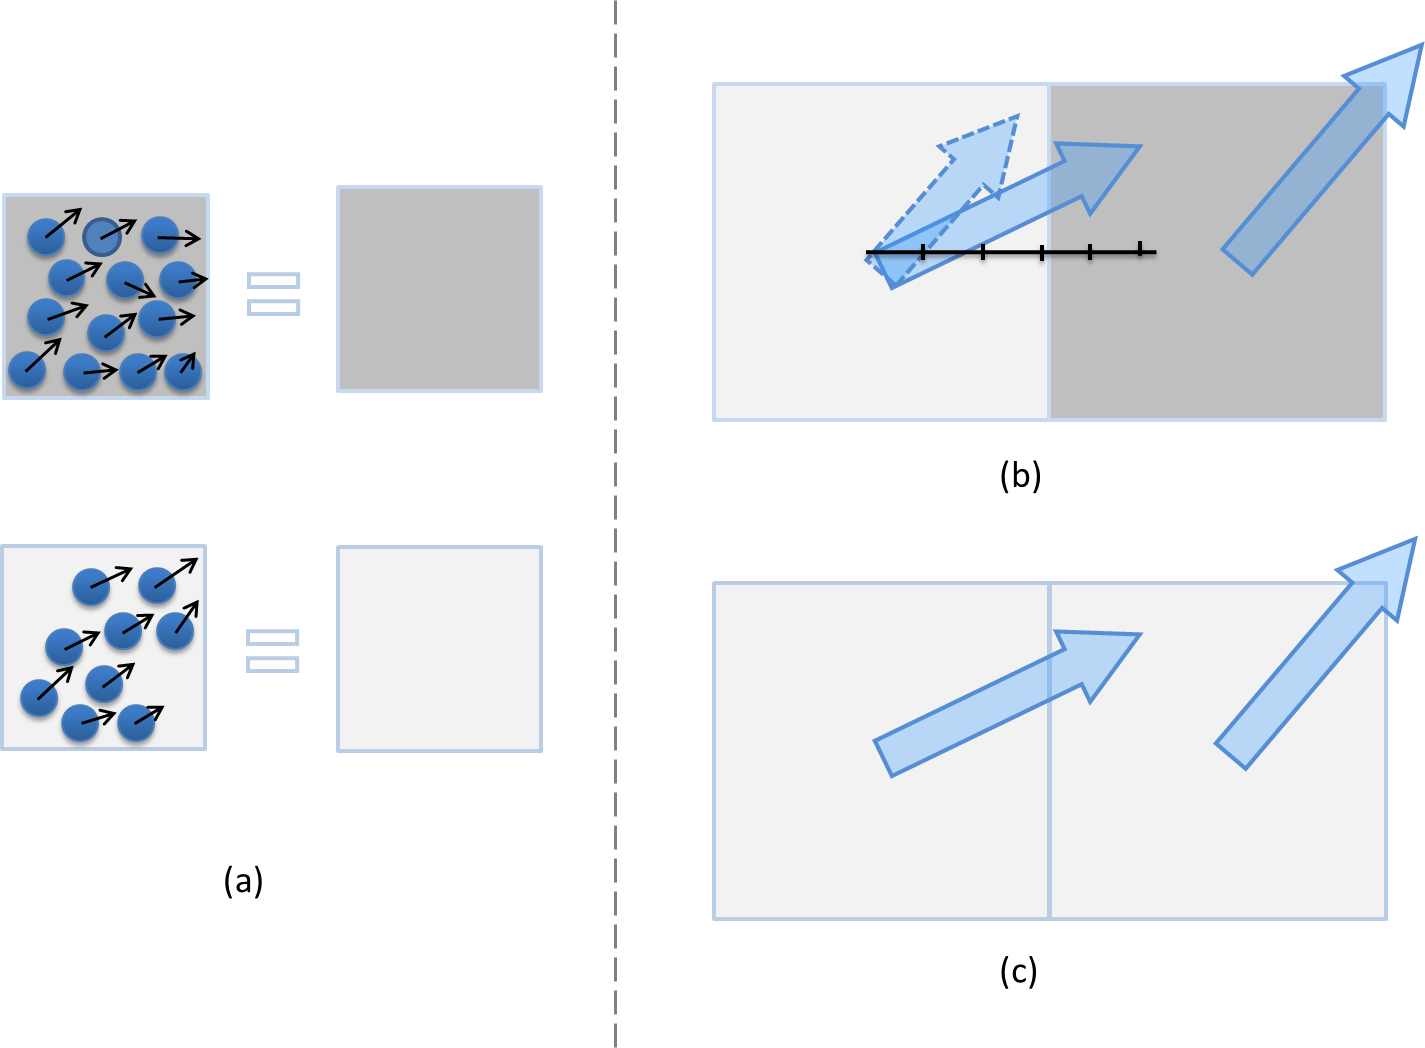
\includegraphics[width=3in]{images/fig_inter_grid_constraints}
  \caption{Illustration of maximum grid density constraints. Image (a) is the transfering process from discrete agent information to continuous representation. Dark gray grids mean maximum density while light gray grids mean lower density. In image (b), the right grid is full of agents and becomes imcompressible. The velocity of left grid on x axis couldn't be larger than the right grid's. In image(c), both grids are not in maximum density means the velocity is not constrained.}
  \label{figure:grid_constraints}
\end{figure}

While trying to reach the minimal energy cost of inter-group collision, we should also keep the density of each group below the maximum density $\rho_{max}$ because of the incompressibility of human body. If the density of the grid $i$ is below $\rho_{max}$, agents can be pushed into the grid from neighbor grids. When the density of the grid $i$ is greater than $\rho_{max}$, the the grid is incompressible. The smooth term should be,
\begin{equation}
\label{eq:7}
V(\left|l_i,l_j\right|) = \left\{ 
{\begin{array}
{*{20}{c}}
{\alpha \left| {{l_i} - {l_j}} \right|,  {\rho _i} \le {\rho _{max}}}\\
{\Delta _{max},  {\rho _i} > {\rho _{max}}}
\end{array}} 
\right.
\end{equation}
where $\Delta_{max}$ is a constant value as a penalty of labels which could lead to potentially overcrowded (see in Figure \ref{figure:grid_constraints}).

%-------------------------------------------------------------------------
\section{Hybrid Crowd Simulation}
\label{section:4}

Continuous crowd methods and agent-based methods are both based on some assumptions about agent number and crowd density. This point of view is also shared by other works like \cite{Golas:2013}. If the assumption of large dense crowd can not hold, collisions between agents and oscillations caused by rearrange process often happen when applying continuous crowd algorithms in low density regions. On the other hand, high density is a nightmare of most agent-based algorithm. Large amount of agent could lead to high computational cost and low frame rate. Further more, for some geometric algorithms like RVO, whose collision avoidance process is based on information from neighbor agents, suffer from the risk failling to find a collision free velocity. 

We addressed the problems by proposing a hybrid model to choose proper algorithm for each group of agents based on the density of the group. There're five steps in our hybrid model pipeline(see in Figure \ref{fig:pipeline}),
\begin{enumerate}
\item Seperate agents into groups, choose continuous or discrete algorithm for groups(see \ref{section:4.1}).
\item Transfer information of agents in dense regions into continuous representation(see \ref{section:3.1}).
\item Reduce inter-group collision and refine group velocities by minimal-energy method(see \ref{section:3.2} and \S\ref{section:3.3})
\item Update velocities of agents in dense region by group velocities(see \ref{section:3.1}) and extract contour and average velocities of dense groups(see \ref{section:4.2}).
\item Add dense groups into agent-based algorithm as moving obstacles and simulate agent-agent and agent-group interactions(see \S\ref{section:4.3}).
\end{enumerate}

\subsection{Crowd Seperation}
\label{section:4.1}

Our crowd seperation method are based on group densities from \S\ref{section:3.1}. There're two cases for varying densities. For the $i$th grid, if $\rho_i \in [\rho_{min}, \rho_{max}]$, it should be marked as a dense grid and apply continuous algorithm described in \S\ref{section:3}. Otherwise, if $\rho_i \in (0, \rho_{min})$, it should be marked as a sparse grid and apply agent-based algorithm like RVO.

\subsection{Dense Crowd Contour Extraction}
\label{section:4.2}

After crowd seperation, we have a set of dense grids for continuous crowd method and a set of sparse girds for agent-based method. Before we move to the inter-group collision energy minimization step, we should first merge dense grids into several groups by detecting connected components. Then we extract the contour $\mathcal{C}_i$ of each group $\mathcal{G}_i$. As we only need rough contours to support agent-group interactions, we use a simple contour extraction algorithm described below,
\begin{itemize}
\item For each group $\mathcal{G}_i$ DO
\begin{enumerate}
\item Sort agents in group $\mathcal{G}_i$ by its vertical position in ascending order, positions of agents on the top and bottom of the list are marked as $\textbf{p}_{min}$ and $\textbf{p}_{max}$
\item Compute the vertical range $\Delta = \textbf{p}_{max, y} - \textbf{p}_{min, y}$ of the group
\item Divide $\Delta$ into $N$ buckets, $N = {\Delta}/{r}$. Put agents into buckets according to its vertical position
\item For each bucket $j$, sort agents in this bucket by horizontal position in ascending order, and mark the position of agents on the top and bottom of the list are marked as $\textbf{p}_{j, left}$ and $\textbf{p}_{j, right}$.
\item Connect points in such an order: $\textbf{p}_{min}$, $\textbf{p}_{1, left}$, $\textbf{p}_{2, left}$, $\cdots$, $\textbf{p}_{N-1, left}$, $\textbf{p}_{N, left}$, $\textbf{p}_{max}$, $\textbf{p}_{N, right}$, $\textbf{p}_{N-1, right}$, $\cdots$, $\textbf{p}_{2, right}$, $\textbf{p}_{1, right}$ and $\textbf{p}_{min}$ to create a contour polygon $\mathcal{C}_i$.
\end{enumerate}
\item END for loop
\end{itemize}
%and regist these contours as moving obstacles to support interactions between agents and groups(see \S\ref{section:4.3}).  

\subsection{Hybrid Crowds Interaction}
\label{section:4.3}

With agents in low density regions and contours of dense groups, we can simulate agent-agent and agent-group collision avoidance by applying a agent-based algorithm. Here, we use reciprocal velocity obstacle (RVO) algorithm \cite{VDBerg:2008} implemented in the RVO2 library. Before calling RVO to simulate, we add contours of dense groups with a offset $\Delta x = \Delta t \cdot \sum_{i}{\textbf{v}_i}$, and then put the updated contours into RVO as obstacles to support interactions between agents and groups. We define a scale parameter $\mathcal{S}$ as the discomfort distance to control whether the agent prefer to avoid or join a dense group. The obstacle will be a Minkowski sum of the contour with a offset and a circle with radius of $\mathcal{S}$. The simulation of hybrid crowd interactions is illustrated in Figure \ref{fig:agent_group_interaction}.

\begin{figure}

\centering
  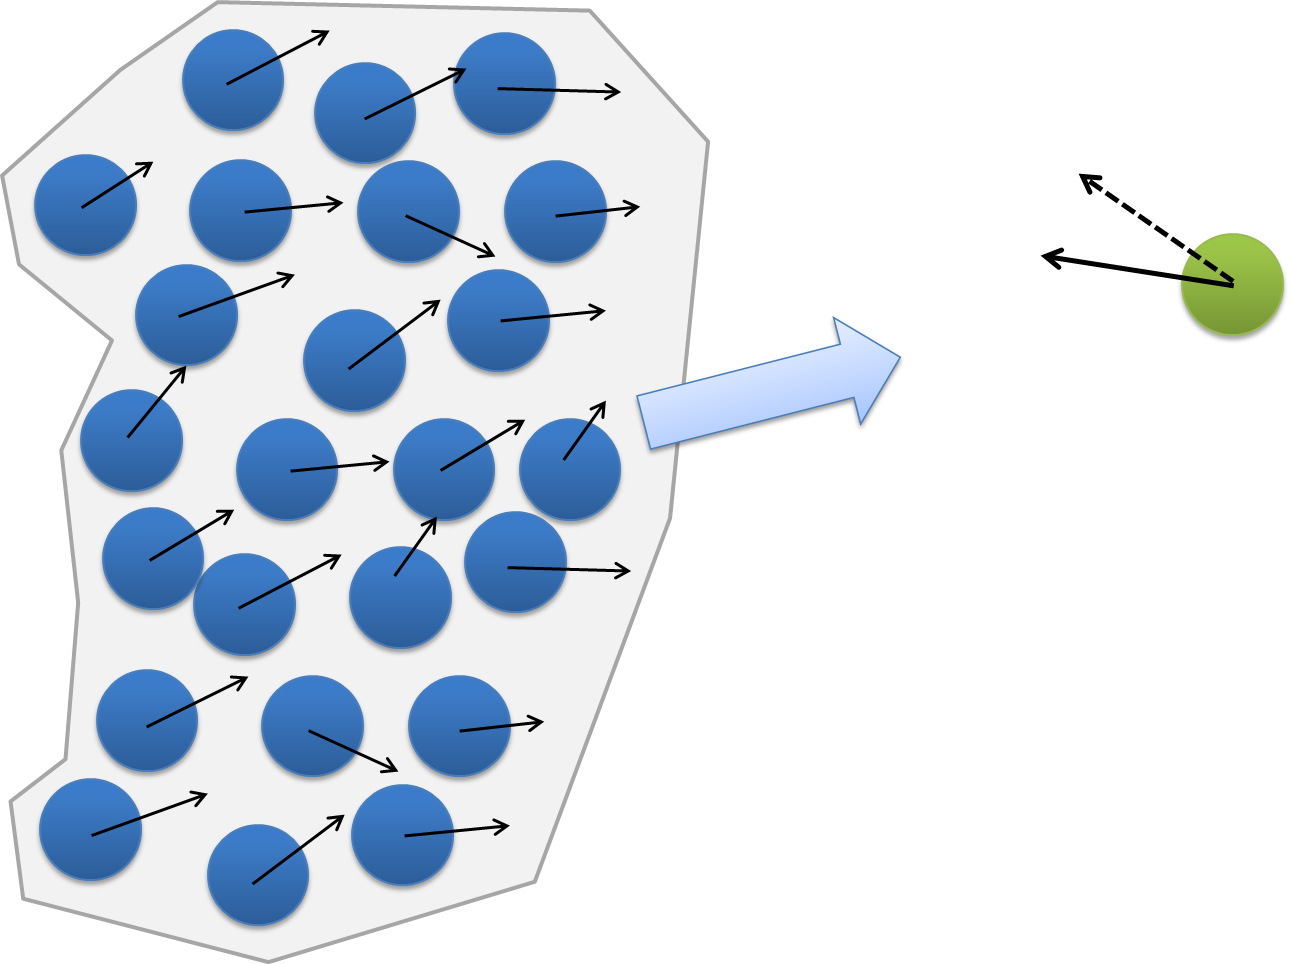
\includegraphics[width=1.6in]{images/agent_group_collision}
  \caption{Illustration of hybrid crowd interactions. The blue agents are in high density region, while the green agents are in low density region. As the contour and average of the dense group is extracted and the group is set as obstacle, the green agent tries to avoid collide with the dense group.}
  \label{fig:agent_group_interaction}
\end{figure}

%-------------------------------------------------------------------------
\section{Results}
\label{section:5}
Our approach was implemented in C/C++. We provide our run-time performance on a Intel Core i7 at 2.9GHz with 4 cases in Table \ref{table:1}. We measured the per frame performance of both agent-based module and continuous module, and the entire hybrid pipeline. From Table \ref{table:1}, we can see that agent-based is the performance bottleneck when there're large amount of agents in the scene. While the agent number is below 10K, our method can reach real-time performance for most cases.

\begin{figure}
  \centering
  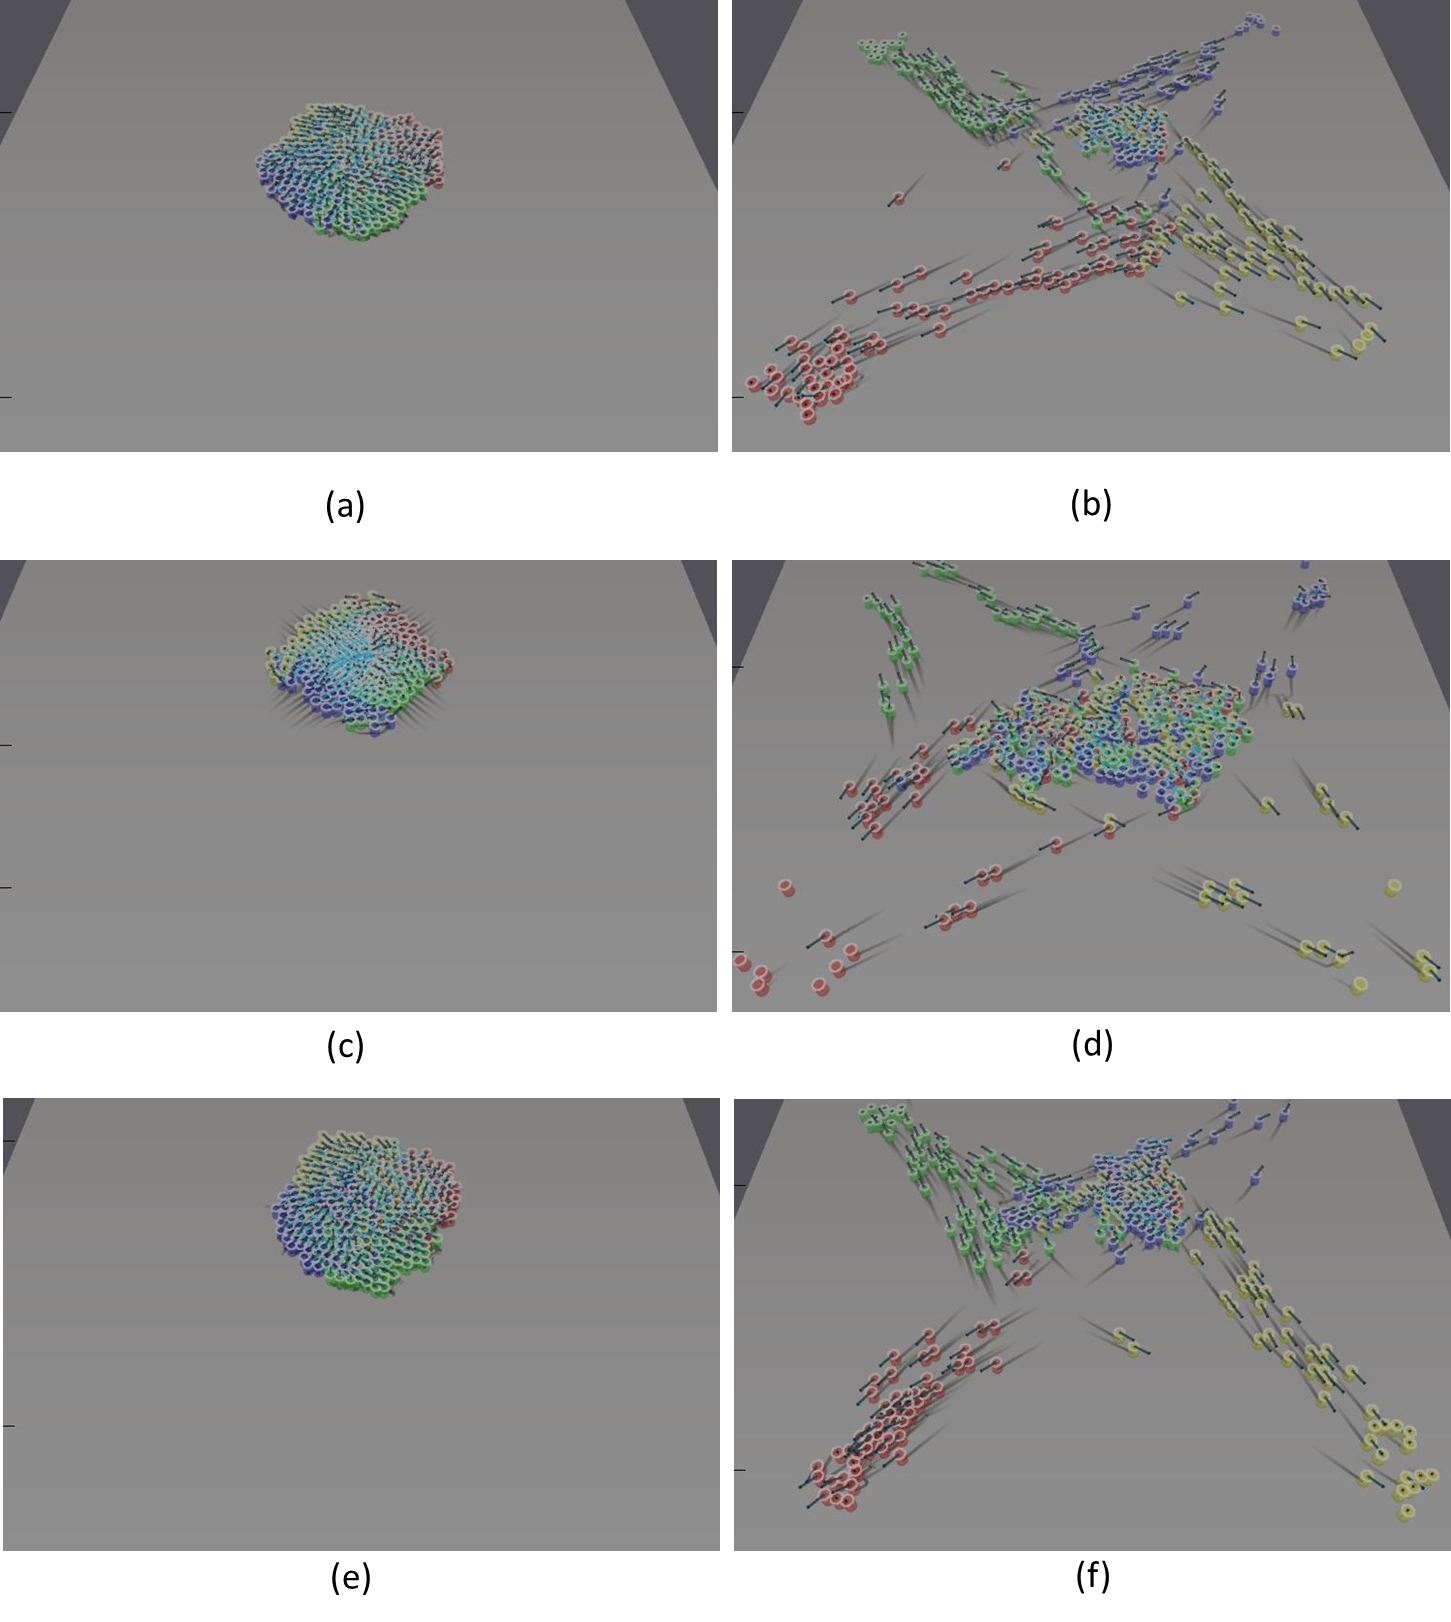
\includegraphics[width=3.2in]{images/four_corner}
  \caption{4 groups of agents crossing the center. The top row is generated by our hybrid pipeline. The middle row is simulated only by RVO algorithm. The bottom row is simulated only by continuous method implemented in our pipeline.}
  \label{fig:four_corner}
\end{figure}

\begin{figure}
  \centering
  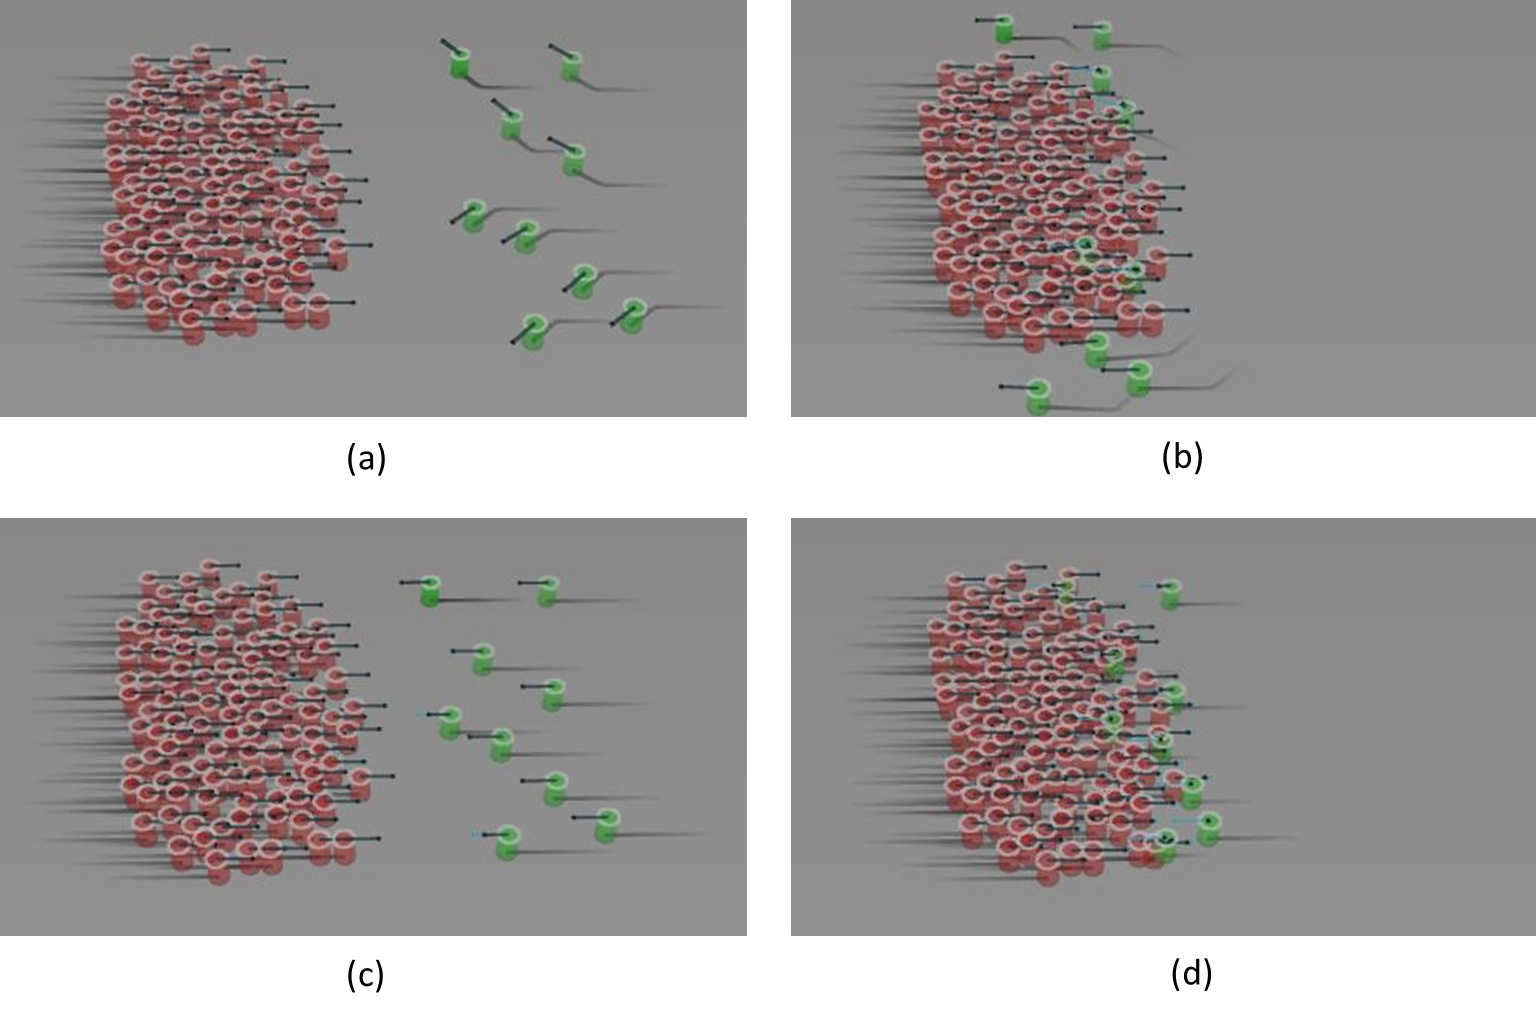
\includegraphics[width=3.2in]{images/cross}
  \caption{Interaction between agents and groups. There're two groups of agents crossing the center. The left(red) group is a dense group. The right(green) group is a low density group. The two rows of the image are set by different discomfort distance $\mathcal{S}$ of group contour. In the top row, the dense group is considered as a rigid object, the individual agents in green try to avoid collision with the group. In the bottom row, the dense group is considered as a much smaller obstacle than its real size, the individual agents choose to join the group.}
  \label{fig:cross}
\end{figure}

We tested our approach on a number of scenes. The first case shows different performances of our hybrid model, pure agent-based algorithm and pure continuous crowd algorithm, see in Figure \ref{fig:four_corner}. In this case, four groups with same number of people on the four corners of a square, heading towads each other and crossing the center. In the simulation by RVO algorithm, the four groups of people stuck at the center, and only agents on the edge of the crowd can keep moving, while the agents in the hybrid model and continuous crowd algorithm begin to spin as a whole group until each group find path to their goal. The groups in hybrid model and continuous crowd algorithm share similar movement till most agents stop stucking and spinning in the center. Then, the rest agents in the center of hybrid model can get faster to their goal because some of the agents are applied agent-based algorithm and able to avoid the dense groups due to the decrease of the density of the center region.

Our second case shows different behaviors of agent-group interaction with different discomfort distance $\mathcal{S}$ of group contour. From the experiment, we can see that, with greater discomfort distance $\mathcal{S}$ which means a larger obstacle, individual agents are more likely to avoid collision with dense groups. And individual agents are more likely to join dense groups with smaller $\mathcal{S}$.

\begin{table}  
\centering  
\begin{tabular}{|c|c|c|c|}
\hline 
Scene & \# Agent & Modules & Time(ms) \\ 
\hline 
Crossing & 500 & Agent-based & 0.7 \textasciitilde 3.8 \\ 
 &  & Continuous & 0.2 \textasciitilde 2.7 \\ 
 &  & Total Hybrid & 1.1 \textasciitilde 6.9 \\ 
\hline 
4 Groups & 4000 & Agent-based & 6.6 \textasciitilde 22.1 \\ 
 &  & Continuous & 24.2 \textasciitilde 42.5 \\ 
 &  & Total Hybrid & 37.4 \textasciitilde 49.0 \\ 
\hline 
4 Groups L & 10000 & Agent-based & 60.7 \textasciitilde 373.4 \\ 
 &  & Continuous & 36.6 \textasciitilde 61.5 \\ 
 &  & Total Hybrid & 107.3 \textasciitilde 379.5 \\ 
\hline 
4 Groups XL & 25000 & Agent-based & 0.7 \textasciitilde 436.1 \\ 
 &  & Continuous & 25.7 \textasciitilde 170 \\  
 &  & Total Hybrid & 143.7 \textasciitilde 480.3 \\ 
\hline 
\end{tabular} 
\caption{Performance of our method}  
\label{table:1}
\end{table}
%-------------------------------------------------------------------------
\section{Conclusion}
In this paper, we present a hybrid model to simulate varying densities crowd. We define three types of interactions in crowd behaviors, agent-agent interaction, agent-group interaction and group-group interaction. Our hybrid model enables the simulation of more realistic crowd movement with combinations of the three interactions, especially the agent-group interaction which is first introduced in crowd simulation. Finally, we formulate and develop our minimal-energy model to reduce collision energy between dense groups. 

There're some limitation in our approach. First, because the formulation of energy model are based on Graph-Cut algorithm, we're using discrete value to represent a continuous interval. We're looking for interpolation methods to provide continuous value for energy model. Secondly, our pipeline is not parallelize implemented which limits our performance. GPU based implementation are needed in our future work. 

%-------------------------------------------------------------------------
%\bibliographystyle{eg-alpha}
\bibliographystyle{eg-alpha-doi}

\bibliography{reference}
\end{document}
